\chapter{Binäärihakupuu}

Binäärihakupuu on tietorakenne, joka pitää yllä
alkioiden joukkoa, samaan tapaan kuin hajautustaulu.
Binäärihakupuuta käyttäen joukon operaatiot vievät aikaa $O(\log n)$
kaikissa tapauksissa.
Käytännössä binäärihakupuu toimii yleensä hieman hitaammin
kuin hajautustaulu, mutta toisaalta siinä ei ole riskinä,
että operaatiot veisivät koskaan aikaa $O(n)$.

Binäärihakupuun tärkein etu hajautustauluun verrattuna on kuitenkin,
että se säilyttää joukon alkioita \emph{järjestyksessä}.
Tämän ansiosta voimme toteuttaa tehokkaasti
esimerkiksi seuraavat operaatiot:

\begin{itemize}
\item etsi joukon pienin/suurin alkio
\item etsi joukon pienin alkio, joka on vähintään $x$
\item etsi joukon suurin alkio, joka on enintään $x$
\end{itemize}

Hajautustaulu \emph{ei} pysty tarjoamaan näitä operaatioita tehokkaasti,
koska alkiot ovat siinä sekalaisessa järjestyksessä.
Jos tarvitsemme näitä operaatioita,
meidän tuleekin käyttää binäärihakupuuta hajautustaulun sijasta.

\section{Taustaa binääripuista}

Binäärihakupuun taustalla on yleisempi tietorakenne \emph{binääripuu}.
Ennen kuin tutustumme binäärihakupuuhun,
meidän onkin hyvä selvittää ensin, mikä on binääripuu ja mitä
ominaisuuksia siihen liittyy.

Binääripuu muodostuu $n$ solmusta, jotka on yhdistetty toisiinsa.
Puussa ylimpänä on solmu, jota kutsutaan \emph{juureksi}.
Jokaisella solmulla voi olla vasen ja oikea \emph{lapsi},
ja kaikilla solmuilla juurta lukuun ottamatta on yksikäsitteinen \emph{vanhempi}.
Puun \emph{lehtiä} ovat solmut, joilla ei ole lapsia.

Binääripuun rakenne on rekursiivinen:
jokainen solmu toimii juurena \emph{alipuulle},
joka on myös binääripuu.
Voimme ajatella, että jokaisessa binääripuun
solmussa vasen ja oikea lapsi on joko tyhjä
tai toinen binääripuu.

\begin{figure}
\center
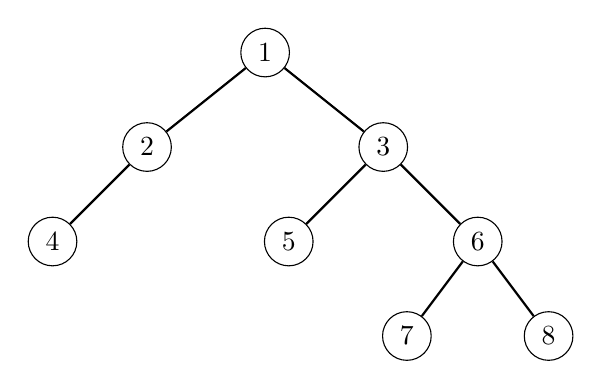
\begin{tikzpicture}[scale=0.6]
\node[draw, circle] (1) at (0,0) {$1$};
\node[draw, circle] (2) at (-2.5,-2) {$2$};
\node[draw, circle] (3) at (2.5,-2) {$3$};
\node[draw, circle] (4) at (-4.5,-4) {$4$};
\node[draw, circle] (5) at (0.5,-4) {$5$};
\node[draw, circle] (6) at (4.5,-4) {$6$};
\node[draw, circle] (7) at (3,-6) {$7$};
\node[draw, circle] (8) at (6,-6) {$8$};
\path[draw,thick,-] (1) -- (2);
\path[draw,thick,-] (1) -- (3);
\path[draw,thick,-] (2) -- (4);
\path[draw,thick,-] (3) -- (5);
\path[draw,thick,-] (3) -- (6);
\path[draw,thick,-] (6) -- (7);
\path[draw,thick,-] (6) -- (8);
\end{tikzpicture}
\caption{Binääripuu, jossa on 8 solmua. Puun juuri on solmu 1,
ja puun lehtiä ovat solmut 4, 5, 7 ja 8.}
\label{fig:binpuu}
\end{figure}

Kuvassa \ref{fig:binpuu} on esimerkki binääripuusta, jossa on 8 solmua.
Solmu 1 on puun juuri, ja solmut 4, 5, 7 ja 8 ovat puun lehtiä.
Solmun 3 vasen lapsi on solmu 5, oikea lapsi on solmu 6
ja vanhempi on solmu 1.
Solmun 3 alipuu sisältää solmut 3, 5, 6, 7 ja 8.

Binääripuun juuren \emph{syvyys} on 0 ja jokaisen muun solmun syvyys on yhtä
suurempi kuin sen vanhemman syvyys.
Binääripuun \emph{korkeus} on puolestaan suurin puun solmussa
esiintyvä syvyys.
Esimerkiksi kuvan \ref{fig:binpuu} puun korkeus on 3,
koska solmujen 7 ja 8 syvyys on 3.

\begin{figure}
\center
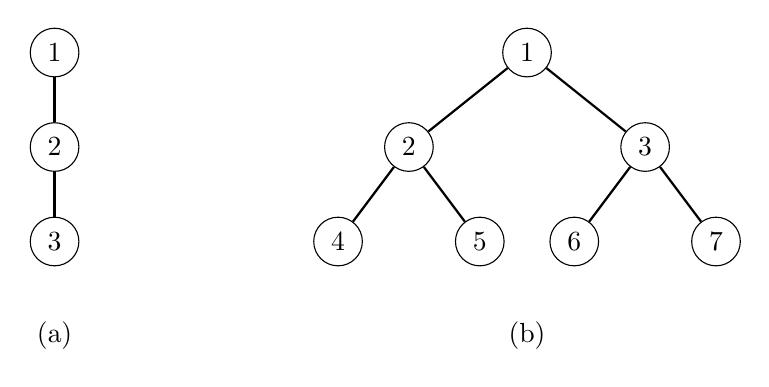
\begin{tikzpicture}[scale=0.6]
\begin{scope}
\node[draw, circle] (1) at (0,0) {$1$};
\node[draw, circle] (2) at (0,-2) {$2$};
\node[draw, circle] (3) at (0,-4) {$3$};
\path[draw,thick,-] (1) -- (2);
\path[draw,thick,-] (2) -- (3);
\node at (0,-6) {(a)};
\end{scope}
\begin{scope}[xshift=10cm]
\node[draw, circle] (1) at (0,0) {$1$};
\node[draw, circle] (2) at (-2.5,-2) {$2$};
\node[draw, circle] (3) at (2.5,-2) {$3$};
\node[draw, circle] (4) at (-4,-4) {$4$};
\node[draw, circle] (5) at (-1,-4) {$5$};
\node[draw, circle] (6) at (1,-4) {$6$};
\node[draw, circle] (7) at (4,-4) {$7$};
\path[draw,thick,-] (1) -- (2);
\path[draw,thick,-] (1) -- (3);
\path[draw,thick,-] (2) -- (4);
\path[draw,thick,-] (2) -- (5);
\path[draw,thick,-] (3) -- (6);
\path[draw,thick,-] (3) -- (7);
\node at (0,-6) {(b)};
\end{scope}
\end{tikzpicture}
\caption{(a) Vähiten solmuja sisältävä korkeuden 2 binääripuu.
(b) Eniten solmuja sisältävä korkeuden 2 binääripuu.}
\label{fig:binraj}
\end{figure}

Jos binääripuun korkeus on $h$, siinä on vähintään $h+1$ solmua,
jolloin puu on pelkkä solmujen lista,
ja enintään $2^{h+1}-1$ solmua,
jolloin kaikilla tasoilla on kaikki mahdolliset solmut.
Kuva \ref{fig:binraj} näyttää esimerkit näistä tapauksista,
kun puun korkeus on $2$.

\subsection{Binääripuun toteutus}

Voimme toteuttaa binääripuun linkitettynä rakenteena niin,
että jokainen puun solmu on olio, josta on viittaus
vasempaan ja oikeaan lapseen.
Javassa voimme määritellä solmua vastaavan luokan seuraavasti:

\begin{code}
public class Solmu {
    Solmu vasen, oikea;
    int arvo;

    public Solmu(Solmu vasen, Solmu oikea, int arvo) {
        this.vasen = vasen;
        this.oikea = oikea;
        this.arvo = arvo;
    }
}
\end{code}

Kentät \texttt{vasen} ja \texttt{oikea} osoittavat solmun
vasempaan ja oikeaan lapseen.
Jos lapsi puuttuu, sen tilalla on arvo \texttt{null}.
Kentässä \texttt{arvo} on puolestaan solmun arvo.
Nyt voimme määritellä kuvan \ref{fig:binpuu} binääripuun näin:

\begin{code}
Solmu s1, s2, s3, s4, s5, s6, s7, s8;
s1 = new Solmu(s2, s3, 1);
s2 = new Solmu(s4, null, 2);
s3 = new Solmu(s5, s6, 3);
s4 = new Solmu(null, null, 4);
s5 = new Solmu(null, null, 5);
s6 = new Solmu(s7, s8, 6);
s7 = new Solmu(null, null, 7);
s8 = new Solmu(null, null, 8);
\end{code}

Voimme toteuttaa monia binääripuun käsittelyyn liittyviä
operaatioita luontevasti rekursiolla.
Esimerkiksi seuraava metodi laskee, montako solmua
sille annetussa puussa on:

\begin{code}
int laskeSolmut(Solmu puu) {
    if (puu == null) return 0;
    return 1 + laskeSolmut(puu.vasen) + laskeSolmut(puu.oikea);
}
\end{code}

Metodille annetaan parametrina solmu,
joka vastaa puun juurta.
Jos puu on tyhjä, siinä ei ole yhtään solmua.
Muuten puussa on juurisolmu sekä vasemman
ja oikean alipuun solmut.
Pystymme laskemaan alipuiden solmut rekursiivisesti
kutsumalla samaa metodia uudestaan.


Seuraava metodi puolestaan selvittää, mikä on puun korkeus.
Huomaa, että jos puu on tyhjä, tulkitsemme,
että sen korkeus on $-1$.

\begin{code}
int korkeus(Solmu puu) {
    if (puu == null) return -1;
    return 1 + Math.max(korkeus(puu.vasen), korkeus(puu.oikea));
}
\end{code}

\subsection{Läpikäyntijärjestykset}

Voimme käydä läpi binääripuun solmut rekursiivisesti
juuresta alkaen.
Solmujen läpikäyntiin on kolme tavallista järjestystä:

\begin{itemize}
\item \emph{esijärjestys}: käsittelemme ensin solmun, sitten vasemman alipuun
ja lopuksi oikean alipuun
\item \emph{sisäjärjestys}: käsittelemme ensin vasemman alipuun, sitten solmun
ja lopuksi oikean alipuun
\item \emph{jälkijärjestys}: käsittelemme ensin vasemman alipuun,
sitten oikean alipuun ja lopuksi solmun
\end{itemize}

Esimerkiksi kuvan \ref{fig:binpuu} puussa
esijärjestys on $[1,2,4,3,5,6,7,8]$,
sisäjärjes\-tys on $[4,2,1,5,3,7,6,8]$ ja
jälkijärjestys on $[4,2,5,7,8,6,3,1]$.

Seuraava metodi tulostaa binääripuun solmut
sisäjärjestyksessä, kun sille annetaan parametrina
puun juuri.

\begin{code}
void tulosta(Solmu puu) {
    if (puu == null) return;
    tulosta(puu.vasen);
    System.out.println(puu.arvo);
    tulosta(puu.oikea);
}
\end{code}

\section{Binäärihakupuun toiminta}

\emph{Binäärihakupuu} on binääripuu, jonka jokaisen solmun
arvona on yksi joukon alkioista.
Jokaisessa solmussa
kaikki alkiot vasemmassa alipuussa ovat pienempiä
kuin solmun alkio ja vastaavasti kaikki alkiot
oikeassa alipuussa ovat suurempia kuin solmun alkio.
Tämän ominaisuuden ansiosta voimme löytää halutun
alkion puusta aloittamalla haun puun juuresta.

\begin{figure}
\center
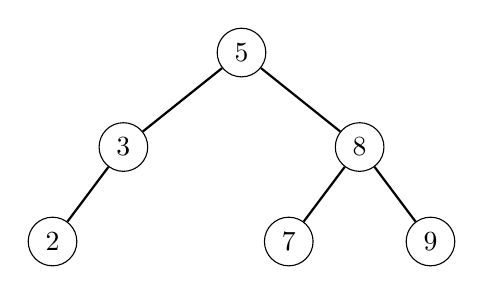
\begin{tikzpicture}[scale=0.6]
\node[draw, circle] (1) at (0,0) {$5$};
\node[draw, circle] (2) at (-2.5,-2) {$3$};
\node[draw, circle] (3) at (2.5,-2) {$8$};
\node[draw, circle] (4) at (-4,-4) {$2$};
\node[draw, circle] (5) at (1,-4) {$7$};
\node[draw, circle] (6) at (4,-4) {$9$};
\path[draw,thick,-] (1) -- (2);
\path[draw,thick,-] (1) -- (3);
\path[draw,thick,-] (2) -- (4);
\path[draw,thick,-] (3) -- (5);
\path[draw,thick,-] (3) -- (6);
\end{tikzpicture}
\caption{Joukkoa $\{2,3,5,7,8,9\}$ vastaava binäärihakupuu.}
\label{fig:bihpuu}
\end{figure}

Kuvassa \ref{fig:bihpuu} on esimerkkinä
joukkoa $\{2,3,5,7,8,9\}$ vastaava binääri\-hakupuu,
jonka juurena on alkio 5.
Vasemmassa alipuussa on kaikki alkiota 5
pienemmät alkiot, eli se vastaa joukkoa $\{2,3\}$.
Oikeassa alipuussa taas on kaikki alkiota 5
suuremmat alkiot, eli se vastaa joukkoa $\{7,8,9\}$.
Huomaa, että tämä on yksi monista tavoista muodostaa
binäärihakupuu joukolle ja voisimme valita myös
minkä tahansa toisen alkion puun juureksi.

\subsection{Operaatioiden toteutus}

Seuraavaksi käymme läpi, kuinka voimme toteuttaa
joukko-operaatioita bi\-näärihakupuun avulla.
Osoittautuu, että voimme toteuttaa kaikki
operaatiot ajassa $O(h)$, missä $h$ on puun korkeus.

\subsubsection{Alkion etsiminen}

Kun haluamme etsiä joukosta alkiota $x$, lähdemme liikkeelle
puun juuresta ja kuljemme alaspäin puussa.
Kun olemme solmussa, jossa on alkio $a$,
vaihtoehtoja on kolme.
Jos $a=x$, olemme löytäneet halutun alkion,
jos $a>x$, jatkamme hakua solmun vasempaan lapseen,
ja jos $a<x$, jatkamme hakua solmun oikeaan lapseen.
Jos kuitenkaan solmulla ei ole lasta,
johon meidän tulisi edetä, toteamme,
että joukossa ei ole alkiota $x$.

\begin{figure}
\center
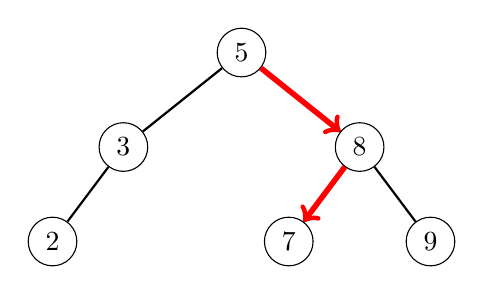
\begin{tikzpicture}[scale=0.6]
\node[draw, circle] (1) at (0,0) {$5$};
\node[draw, circle] (2) at (-2.5,-2) {$3$};
\node[draw, circle] (3) at (2.5,-2) {$8$};
\node[draw, circle] (4) at (-4,-4) {$2$};
\node[draw, circle] (5) at (1,-4) {$7$};
\node[draw, circle] (6) at (4,-4) {$9$};
\path[draw,thick,-] (1) -- (2);
\path[draw,thick,-] (1) -- (3);
\path[draw,thick,-] (2) -- (4);
\path[draw,thick,-] (3) -- (5);
\path[draw,thick,-] (3) -- (6);
\path[draw,thick,red,line width=2pt,->] (1) -- (3);
\path[draw,thick,red,line width=2pt,->] (3) -- (5);
\end{tikzpicture}
\caption{Alkion $7$ etsiminen joukosta $\{2,3,5,7,8,9\}$ juuresta alkaen.}
\label{fig:bihets}
\end{figure}

Kuva \ref{fig:bihets} näyttää, kuinka löydämme alkion 7
joukosta $\{2,3,5,7,8,9\}$.
Juurena on alkio 5, joten alkion 7 täytyy olla juuren
oikeassa alipuussa.
Tämän alipuun juurena on alkio 8,
joten nyt taas tiedämme, että alkion 7 täytyy olla
vasemmassa alipuussa, josta se löytyykin.

\subsubsection{Alkion lisääminen}

Kun haluamme lisätä joukkoon alkion $x$,
jota ei vielä ole joukossa, kuljemme ensin
puussa aivan kuin etsisimme alkiota $x$.
Sitten kun olemme päässeet solmuun,
jolla ei ole lasta, johon meidän tulisi edetä,
luomme uuden solmun alkiolle $x$ ja lisäämme
sen tähän kohtaan lapseksi.

\begin{figure}
\center
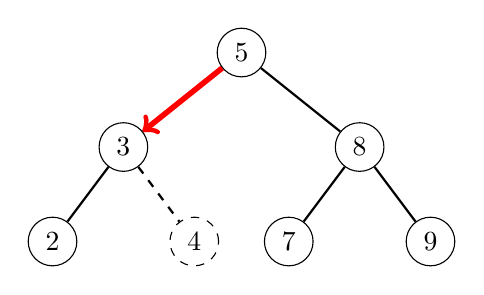
\begin{tikzpicture}[scale=0.6]
\node[draw, circle] (1) at (0,0) {$5$};
\node[draw, circle] (2) at (-2.5,-2) {$3$};
\node[draw, circle] (3) at (2.5,-2) {$8$};
\node[draw, circle] (4) at (-4,-4) {$2$};
\node[draw, circle] (5) at (1,-4) {$7$};
\node[draw, circle] (6) at (4,-4) {$9$};
\node[draw, circle, dashed] (7) at (-1,-4) {$4$};
\path[draw,thick,-] (1) -- (2);
\path[draw,thick,-] (1) -- (3);
\path[draw,thick,-] (2) -- (4);
\path[draw,thick,-] (3) -- (5);
\path[draw,thick,-] (3) -- (6);
\path[draw,thick,dashed,-] (2) -- (7);
\path[draw,thick,red,line width=2pt,->] (1) -- (2);
\end{tikzpicture}
\caption{Alkion 4 lisääminen joukkoon $\{2,3,5,7,8,9\}$.}
\label{fig:bihpu2}
\end{figure}

Kuva \ref{fig:bihpu2} näyttää, kuinka lisäämme alkion 4
joukkoon $\{2,3,5,7,8,9\}$.
Kun haemme puusta solmua 4, päädymme solmuun 3,
jolla ei ole oikeaa lasta.
Niinpä lisäämme solmun 4 solmun 3 oikeaksi lapseksi.

\subsubsection{Pienin alkio / suurin alkio}

Kun haluamme löytää joukon pienimmän alkion,
lähdemme liikkeelle juuresta ja etenemme joka askeleella
solmun vasempaan lapseen.
Kun solmulla ei ole enää vasenta lasta,
olemme löytäneet joukon pienimmän alkion.

Vastaavalla tavalla löydämme joukon suurimman alkion
etenemällä koko ajan oikeaan lapseen juuresta.

\subsubsection{Seuraava suurempi alkio / edellinen pienempi alkio}

Kun haluamme löytää joukon pienimmän alkion,
joka on suurempi kuin $x$,
lähdemme liikkeelle puun juuresta.
Kun olemme solmussa, jossa on alkio $a$,
etenemme vasempaan lapseen,
jos $a>x$, ja oikeaan lapseen, jos $a \le x$.
Jatkamme näin, kunnes emme voi edetä alemmas.
Haluttu alkio on pienin alkiota $x$ suurempi alkio
kaikista alkioista, joiden kautta kuljimme.

Kun haluamme vastaavasti löytää joukon suurimman alkion,
joka on pienempi kuin $x$,
menettelemme käänteisesti edelliseen nähden.

\subsubsection{Alkion poistaminen}

Kun haluamme poistaa joukosta alkion $x$, etsimme ensin
alkiota $x$ vastaavan solmun tavalliseen tapaan.
Jos solmulla ei ole lapsia tai vain yksi lapsi,
meidän on helppoa poistaa solmu puusta ja säilyttää
puun rakenne muuten ennallaan.
Jos kuitenkin solmulla on kaksi lasta,
tilanne on hankalampi.
Tällöin etsimme alkion $y$,
joka on pienin $x$:ää suurempi alkio,
ja vaihdamme keskenään alkiot $x$ ja $y$ puussa.
Tämän jälkeen meidän on helppoa poistaa solmu,
jossa on nyt alkio $x$,
koska sillä ei voi olla kahta lasta
(koska jos solmulla olisi vasen lapsi,
$y$ ei olisi pienin $x$:ää suurempi alkio).

\begin{figure}
\center
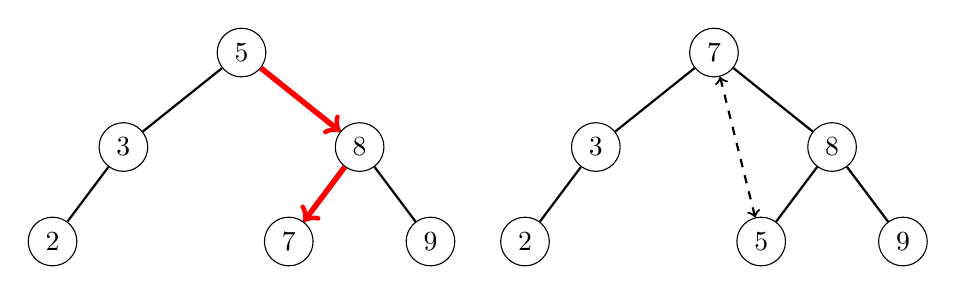
\begin{tikzpicture}[scale=0.6]
\begin{scope}
\node[draw, circle] (1) at (0,0) {$5$};
\node[draw, circle] (2) at (-2.5,-2) {$3$};
\node[draw, circle] (3) at (2.5,-2) {$8$};
\node[draw, circle] (4) at (-4,-4) {$2$};
\node[draw, circle] (5) at (1,-4) {$7$};
\node[draw, circle] (6) at (4,-4) {$9$};
\path[draw,thick,-] (1) -- (2);
\path[draw,thick,-] (1) -- (3);
\path[draw,thick,-] (2) -- (4);
\path[draw,thick,-] (3) -- (5);
\path[draw,thick,-] (3) -- (6);
\path[draw,thick,red,line width=2pt,->] (1) -- (3);
\path[draw,thick,red,line width=2pt,->] (3) -- (5);
\end{scope}
\begin{scope}[xshift=10cm]
\node[draw, circle] (1) at (0,0) {$7$};
\node[draw, circle] (2) at (-2.5,-2) {$3$};
\node[draw, circle] (3) at (2.5,-2) {$8$};
\node[draw, circle] (4) at (-4,-4) {$2$};
\node[draw, circle] (5) at (1,-4) {$5$};
\node[draw, circle] (6) at (4,-4) {$9$};
\path[draw,thick,-] (1) -- (2);
\path[draw,thick,-] (1) -- (3);
\path[draw,thick,-] (2) -- (4);
\path[draw,thick,-] (3) -- (5);
\path[draw,thick,-] (3) -- (6);
\path[draw,thick,<->,dashed] (1) -- (5);
\end{scope}
\end{tikzpicture}
\caption{Alkion 5 poistaminen joukosta $\{2,3,5,7,8,9\}$. (a) Koska alkiolla
5 on kaksi lasta, etsimme seuraavan suuremman alkion 7.
(b) Vaihdamme keskenään alkiot 5 ja 7, minkä jälkeen voimme poistaa helposti alkion 5.}
\label{fig:bihpu3}
\end{figure}

Kuva \ref{fig:bihpu3} näyttää, kuinka poistamme joukosta $\{2,3,5,7,8,9\}$ alkion 5.
Alkio on puun juuressa ja solmulla on kaksi lasta,
joten meidän tulee etsiä ensin pienin alkiota 5 suurempi alkio,
joka on 7.
Vaihdamme sitten keskenään arvot 5 ja 7,
minkä jälkeen meidän on helppoa poistaa alkio 5.

\subsection{Operaatioiden tehokkuus}

Binäärihakupuun operaatiot vievät aikaa $O(h)$,
missä $h$ on puun korkeus, joten operaatioiden tehokkuus
riippuu puun korkeudesta.
Niinpä operaatioiden tehokkuuteen vaikuttaa, miten olemme
rakentaneet puun.
Esimerkiksi kuvassa \ref{fig:bihkor} on kaksi mahdollista
binäärihakupuuta joukolle $\{1,2,3,4,5\}$.
Vasemman puun korkeus on 2, kun taas oikean puun korkeus on 4.

\begin{figure}
\center
\begin{tikzpicture}[scale=0.6]
\begin{scope}
\node[draw, circle] (1) at (0,0) {$1$};
\node[draw, circle] (2) at (1,-2) {$2$};
\node[draw, circle] (3) at (2,-4) {$3$};
\node[draw, circle] (4) at (3,-6) {$4$};
\node[draw, circle] (5) at (4,-8) {$5$};
\path[draw,thick,-] (1) -- (2);
\path[draw,thick,-] (2) -- (3);
\path[draw,thick,-] (3) -- (4);
\path[draw,thick,-] (4) -- (5);
\end{scope}
\begin{scope}[xshift=-8cm]
\node[draw, circle] (1) at (0,0) {$1$};
\node[draw, circle] (2) at (-2,-2) {$2$};
\node[draw, circle] (3) at (2,-2) {$3$};
\node[draw, circle] (4) at (-4,-4) {$4$};
\node[draw, circle] (5) at (0,-4) {$5$};
\path[draw,thick,-] (1) -- (2);
\path[draw,thick,-] (1) -- (3);
\path[draw,thick,-] (2) -- (4);
\path[draw,thick,-] (2) -- (5);
\end{scope}
\end{tikzpicture}
\caption{Kaksi binäärihakupuuta joukolle $\{1,2,3,4,5\}$.
Vasemman puun korkeus on 2 ja oikean puun korkeus on 4.}
\label{fig:bihkor}
\end{figure}

Jotta binäärihakupuu toimii tehokkaasti, haluamme,
että puun korkeus ei kasva liian suureksi.
Tarkemmin ottaen tavoitteemme on, että
solmut ovat jakautuneet tasaisesti puun eri puolille
ja puun korkeus on $O(\log n)$.
Tällöin sanomme, että puu on \emph{tasapainoinen}.
Jos onnistumme tässä, kaikki puun operaatiot toimivat
tehokkaasti ajassa $O(\log n)$.
Saavutamme tavoitteemme
lisäämällä puuhun ehtoja, jotka rajoittavat
sen korkeutta sopivasti.

Binäärihakupuun tasapainottamiseen tunnetaan monia menetelmiä.
Tutustumme seuraavaksi AVL-puuhun, joka on 
varhaisin tunnettu tasapainoinen binäärihakupuu.
AVL-puu on yksinkertaisempi kuin monet myöhemmin
kehitetyt rakenteet, minkä vuoksi se sopii hyvin esittelemään
puiden tasapainotuksen ideoita.
Javan ja muiden ohjelmointikielten standardikirjastoissa
käyte\-tään kuitenkin muita rakenteita, kuten punamustaa puuta.

\section{AVL-puu}

\emph{AVL-puu} on tasapainoinen binäärihakupuu, jonka
korkeus on aina $O(\log n)$, minkä ansiosta puun operaatiot
toimivat tehokkaasti ajassa $O(\log n)$.
AVL-puussa jokaiseen solmuun liittyy \emph{tasapainoehto},
joka takaa, että puu on tasapainoinen.
Kun päivitämme puuta, meidän täytyy pitää huolta siitä,
että tasapainoehto säilyy voimassa kaikissa solmuissa.

\subsection{Tasapainoehto}

AVL-puun tasapainoehtona on, että
jokaisessa solmussa vasemman ja oikean lapsen alipuiden korkeusero 
on enintään 1.

Esimerkiksi kuvan \ref{fig:bihkor} vasen puu on
AVL-puu, kun taas oikea puu ei ole.
Oikea puu ei ole AVL-puu, koska esimerkiksi solmussa 1
vasemman lapsen alipuun korkeus on $-1$ mutta oikean lapsen
alipuun korkeus on 3.
Korkeuksien erona on siis 4, vaikka ero saisi olla enintään 1.

Kutsumme AVL-puun tasapainoehtoa \emph{AVL-ehdoksi}.
Osoittautuu, että jos binäärihakupuu täyttää AVL-ehdon,
sen korkeus on $O(\log n)$.
Eli jos pystymme toteuttamaan puun operaatiot niin,
että AVL-ehto säilyy, saamme aikaan binäärihakupuun,
jonka operaatiot toimivat ajassa $O(\log n)$.

\begin{figure}
\center
\scriptsize
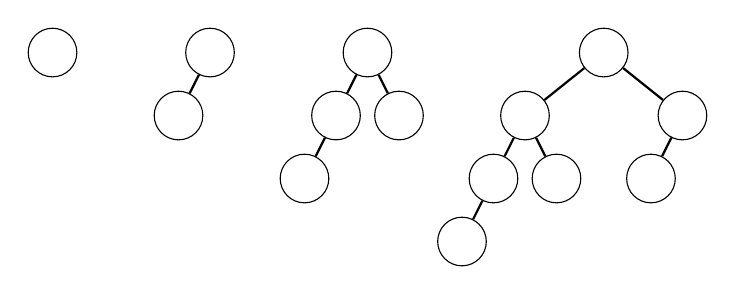
\begin{tikzpicture}[scale=0.4]
\begin{scope}
\node[draw, circle] (2) at (-2.5,-2) {\phantom{$1$}};
\end{scope}
\begin{scope}[xshift=5cm]
\node[draw, circle] (2) at (-2.5,-2) {\phantom{$1$}};
\node[draw, circle] (4) at (-3.5,-4) {\phantom{$1$}};
\path[draw,thick,-] (2) -- (4);
\end{scope}
\begin{scope}[xshift=10cm]
\node[draw, circle] (2) at (-2.5,-2) {\phantom{$1$}};
\node[draw, circle] (4) at (-3.5,-4) {\phantom{$1$}};
\node[draw, circle] (5) at (-1.5,-4) {\phantom{$1$}};
\node[draw, circle] (7) at (-4.5,-6) {\phantom{$1$}};
\path[draw,thick,-] (2) -- (4);
\path[draw,thick,-] (2) -- (5);
\path[draw,thick,-] (4) -- (7);
\end{scope}
\begin{scope}[xshift=15cm,yshift=-2cm]
\node[draw, circle] (1) at (0,0) {\phantom{$1$}};
\node[draw, circle] (2) at (-2.5,-2) {\phantom{$1$}};
\node[draw, circle] (3) at (2.5,-2) {\phantom{$1$}};
\node[draw, circle] (4) at (-3.5,-4) {\phantom{$1$}};
\node[draw, circle] (5) at (-1.5,-4) {\phantom{$1$}};
\node[draw, circle] (6) at (1.5,-4) {\phantom{$1$}};
\node[draw, circle] (7) at (-4.5,-6) {\phantom{$1$}};
\path[draw,thick,-] (1) -- (2);
\path[draw,thick,-] (1) -- (3);
\path[draw,thick,-] (2) -- (4);
\path[draw,thick,-] (2) -- (5);
\path[draw,thick,-] (3) -- (6);
\path[draw,thick,-] (4) -- (7);
\end{scope}
\end{tikzpicture}
\caption{Vähiten solmuja sisältävät AVL-puut korkeuksille 0, 1, 2 ja 3.}
\label{fig:avlkor}
\end{figure}

Miksi sitten AVL-ehto takaa, että binäärihakupuun korkeus
on $O(\log n)$?
Voimme lähestyä asiaa pahimman tapauksen kautta:
kun tiedämme, että AVL-puussa on $n$ solmua,
mikä on sen \emph{suurin mahdollinen} korkeus?
Voimme selvittää tämän tutkimalla käänteisesti,
mikä on \emph{pienin mahdollinen} solmujen määrä
AVL-puussa, jonka korkeus on $h$.

Merkitään $f(h)$:lla korkeutta $h$ olevan AVL-puun
pienintä mahdollista solmujen määrää.
Kuvan \ref{fig:avlkor} mukaisesti funktion ensimmäiset arvot
ovat $f(0)=1$, $f(1)=2$, $f(2)=4$ ja $f(3)=7$.
Yleisemmin
\[f(h)=1+f(h-1)+f(h-2),\]
kun $h \ge 2$, koska jos haluamme rakentaa AVL-puun korkeutta $h$,
jossa on mahdollisimman vähän solmuja,
meidän kannattaa laittaa juuren lapsiksi AVL-puut
korkeutta $h-1$ ja $h-2$ niin,
että kummassakin alipuussa on mahdollisimman vähän solmuja.
Funktiolle pätee
\[f(h) \ge 2 f(h-2),\]
eli funktion arvo ainakin kaksinkertaistuu kahden askeleen välein.
Voimme ilmaista tämän alarajan
\[f(h) \ge 2^{h/2},\]
jonka voimme taas muuttaa ylärajaksi
\[ h \le 2 \log_2 f(h).\]

Tarkastellaan sitten puuta, jossa on $n$ solmua
ja jonka korkeus on $h$.
Korkeudelle täytyy päteä $f(h) \le n$,
koska korkeutta $h$ olevassa puussa on vähintään $f(h)$ solmua.
Niinpä saamme ylärajan
\[h \le 2 \log_2 n,\]
mikä tarkoittaa samaa kuin $h = O(\log n)$.

\subsection{Kiertojen toteutus}

\begin{figure}
\center
\begin{tikzpicture}[scale=0.6]
\newcommand\alipuu[3]{
\path[draw,thick,-] (0+#1,0+#2) -- (-1+#1,-2+#2) -- (1+#1,-2+#2) -- (0+#1,0+#2);
\node at (0+#1,-1.25+#2) {#3};
}
\draw[thick,<->] (5,-2) -- (7,-2);
\begin{scope}
\node[draw, circle] (1) at (0,0) {$x$};
\node[draw, circle] (2) at (2,-2) {$y$};
\alipuu{-2}{-1.5}{$A$}
\alipuu{0.75}{-3.5}{$B$}
\alipuu{3.25}{-3.5}{$C$}
\path[draw,thick,-] (1) -- (2);
\path[draw,thick,-] (1) -- (-2,-1.5);
\path[draw,thick,-] (2) -- (0.75,-3.5);
\path[draw,thick,-] (2) -- (3.25,-3.5);
\end{scope}
\begin{scope}[xshift=10cm]
\node[draw, circle] (1) at (0,-2) {$x$};
\node[draw, circle] (2) at (2,0) {$y$};
\alipuu{-1.25}{-3.5}{$A$}
\alipuu{1.25}{-3.5}{$B$}
\alipuu{4}{-1.5}{$C$}
\path[draw,thick,-] (1) -- (2);
\path[draw,thick,-] (1) -- (-1.25,-3.5);
\path[draw,thick,-] (1) -- (1.25,-3.5);
\path[draw,thick,-] (2) -- (4,-1.5);
\end{scope}
\end{tikzpicture}
\caption{Kierrot, joiden avulla korjaamme AVL-puuta.}
\label{fig:avlkie}
\end{figure}

Voimme toteuttaa AVL-puun operaatiot muuten samaan tapaan
kuin yleisessä binäärihakupuussa, mutta meidän täytyy varmistaa
alkion lisäämisen ja poistamisen jälkeen, että AVL-ehto
on edelleen voimassa.
Tämä onnistuu tekemällä sopivia \emph{kiertoja},
jotka muuttavat puun rakennetta.

Osoittautuu, että voimme korjata puun rakenteen kaikissa
tilanteessa käyttäen kahta kiertotyyppiä,
jotka on esitetty kuvassa \ref{fig:avlkie}.
Puissa $x$ ja $y$ ovat kaksi solmua
ja $A$, $B$ ja $C$ ovat niihin liittyvät alipuut.
Voimme tehdä kierron joko vasemmasta puusta oikeaan puuhun
tai päinvastoin ja vaihtaa tällä tavalla solmujen järjestystä.

\begin{figure}
\center
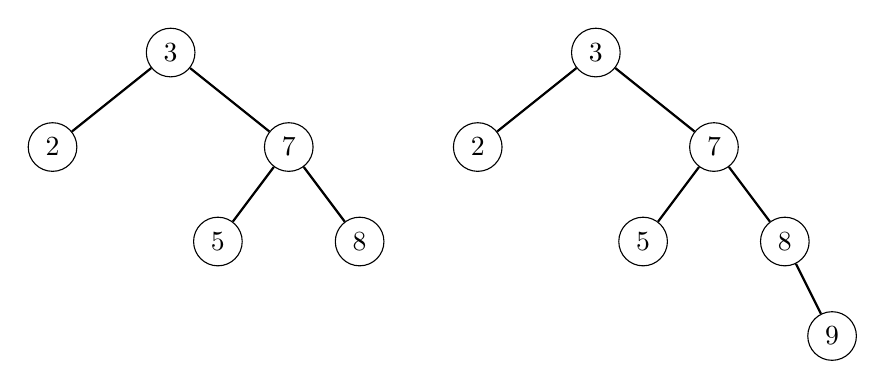
\begin{tikzpicture}[scale=0.6]
\begin{scope}
\node[draw, circle] (1) at (0,0) {$3$};
\node[draw, circle] (2) at (-2.5,-2) {$2$};
\node[draw, circle] (3) at (2.5,-2) {$7$};
\node[draw, circle] (5) at (1,-4) {$5$};
\node[draw, circle] (6) at (4,-4) {$8$};
\path[draw,thick,-] (1) -- (2);
\path[draw,thick,-] (1) -- (3);
\path[draw,thick,-] (3) -- (5);
\path[draw,thick,-] (3) -- (6);
\end{scope}
\begin{scope}[xshift=9cm]
\node[draw, circle] (1) at (0,0) {$3$};
\node[draw, circle] (2) at (-2.5,-2) {$2$};
\node[draw, circle] (3) at (2.5,-2) {$7$};
\node[draw, circle] (5) at (1,-4) {$5$};
\node[draw, circle] (6) at (4,-4) {$8$};
\node[draw, circle] (7) at (5,-6) {$9$};
\path[draw,thick,-] (1) -- (2);
\path[draw,thick,-] (1) -- (3);
\path[draw,thick,-] (3) -- (5);
\path[draw,thick,-] (3) -- (6);
\path[draw,thick,-] (6) -- (7);
\end{scope}
\end{tikzpicture}
\caption{AVL-ehto menee rikki, kun lisäämme puuhun solmun 9.}
\label{fig:avlrik}
\end{figure}

Kun lisäämme AVL-puuhun solmun, se voi rikkoa AVL-ehdon,
jos jossain solmussa lasten alipuiden korkeudet ovat ennen lisäämistä
$h$ ja $h+1$ ja lisäämisen jälkeen $h$ ja $h+2$.
Kuva \ref{fig:avlrik} näyttää esimerkin tällaisesta tilanteesta.
Vasemmassa puussa solmun $3$ lasten korkeudet ovat 0 ja 1,
joten AVL-ehto on kunnossa.
Oikeassa puussa olemme lisänneet solmun $9$,
minkä seurauksena solmun $3$ lasten korkeudet ovat 0 ja 2
eikä AVL-ehto enää päde.

\begin{figure}
\center
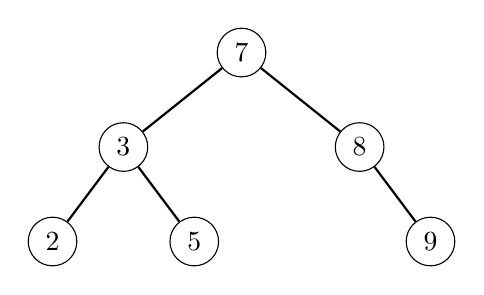
\begin{tikzpicture}[scale=0.6]
\node[draw, circle] (1) at (0,0) {$7$};
\node[draw, circle] (2) at (-2.5,-2) {$3$};
\node[draw, circle] (3) at (2.5,-2) {$8$};
\node[draw, circle] (5) at (-4,-4) {$2$};
\node[draw, circle] (6) at (-1,-4) {$5$};
\node[draw, circle] (7) at (4,-4) {$9$};
\path[draw,thick,-] (1) -- (2);
\path[draw,thick,-] (1) -- (3);
\path[draw,thick,-] (2) -- (5);
\path[draw,thick,-] (2) -- (6);
\path[draw,thick,-] (3) -- (7);
\end{tikzpicture}
\caption{Kierrämme solmun $7$ puun juureksi, jolloin AVL-ehto pätee taas.}
\label{fig:avlkor}
\end{figure}

Korjaamme AVL-ehdon solmun lisäämisen jälkeen
kulkemalla puussa ylös\-päin lisätystä solmusta lähtien,
kunnes tulemme ensimmäiseen solmuun, jossa ehto ei ole voimassa.
Jos tällainen solmu löytyy, palautamme ehdon voimaan tekemällä yhden
tai kaksi kiertoa riippuen lisätyn solmun sijainnista.
Oletetaan, että $x$ on puun alin solmu,
jossa AVL-ehto ei ole voimassa,
$y$ on $x$:n lapsi, jonka alipuussa on lisätty solmu,
ja $z$ on $y$:n lapsi, jonka alipuussa on lisätty solmu.
Tapauksia on kaksi: jos $y$ ja $z$ ovat molemmat
vasempia lapsia tai molemmat oikeita lapsia,
kierrämme solmua $y$ kerran ylöspäin,
ja muuten kierrämme solmua $z$ kahdesti ylöspäin.
Tämän korjauksen jälkeen AVL-ehto on jälleen
voimassa kaikissa puun solmuissa, eli meidän riittää aina
korjata ehto alimmassa solmussa, jossa se ei ole voimassa.

Kuvassa \ref{fig:avlrik} AVL-ehto ei ole voimassa solmussa $3$,
joten $x=3$, $y=7$ ja $z=8$.
Koska $y$ on $x$:n oikea lapsi ja $z$ on $y$:n oikea lapsi,
meidän riittää tehdä yksi kierto, joka nostaa solmua $7$ ylöspäin
puun juureksi.
Tuloksena on kuvan \ref{fig:avlkor} mukainen puu, jossa
AVL-ehto on jälleen voimassa,
koska solmun $7$ kummankin alipuun korkeus on nyt 1.

Kun poistamme puusta solmun, menettelemme melko samalla tavalla
kuin lisäämisessä.
Tässä tapauksessa on mahdollista, että ennen poistoa
jossakin solmussa lasten alipuiden korkeudet ovat $h$ ja $h-1$
ja poiston jälkeen $h$ ja $h-2$.
Poiston jälkeen nousemme puussa ylöspäin ja jos löydämme
tällaisen solmun, korjaamme ehdon niin, että kummankin alipuun
korkeus on $h-1$.
Toisin kuin lisäämisessä, jatkamme tämän jälkeen ylöspäin
ja korjaamme tarvittaessa ehtoa muissa solmuissa,
koska ehdon korjaaminen yhdessä solmussa saattaa rikkoa
sen jossain ylemmässä solmussa.

Pystymme tekemään korjaukset sekä lisäämisen että poistamisen
jälkeen ajassa $O(\log n)$,
koska puun korkeus on $O(\log n)$ ja jokainen yksittäinen
kierto tapahtuu vakioajassa.
Lisäämisen jälkeen kuljemme puuta ylöspäin $O(\log n)$ askelta
ja teemme enintään kaksi kiertoa.
Poistamisen jälkeen taas kuljemme puuta ylöspäin $O(\log n)$ askelta
ja teemme enintään $O(\log n)$ kiertoa.


\section{Javan rakenteet}

Javan tietorakenteet \texttt{TreeSet} ja \texttt{TreeMap}
pohjautuvat punamustaan puuhun,
joka on AVL-puun tapainen mutta monimutkaisempi
binäärihakupuu.
Ne muistuttavat rakenteita \texttt{HashSet} ja \texttt{HashMap},
mutta erona on, että pystymme lisäksi etsimään
alkioita niiden järjestyksen perusteella.

\subsection{\texttt{TreeSet}-rakenne}

Seuraava koodi luo \texttt{TreeSet}-rakenteen,
joka pitää yllä lukujen joukkoa.
Koodi lisää joukkoon alkioita ja tulostaa sitten sen sisällön.
Huomaa, että tulostuksessa joukon alkiot näkyvät
järjestyksessä pienimmästä suurimpaan, koska
binäärihakupuu pitää niitä järjestyksessä.

\begin{code}
TreeSet<Integer> joukko = new TreeSet<>();
joukko.add(4);
joukko.add(1);
joukko.add(8);
joukko.add(7);
System.out.println(joukko); // [1, 4, 7, 8]
\end{code}

Koska joukko on järjestyksessä, pystymme etsimään tehokkaasti
pienim\-män ja suurimman alkion metodeilla \texttt{first} ja \texttt{last}:

\begin{code}
System.out.println(joukko.first()); // 1
System.out.println(joukko.last()); // 8
\end{code}

Pystymme myös etsimään seuraavan tiettyä alkiota
suuremman tai pienemmän alkion metodeilla \texttt{higher} ja \texttt{lower}:

\begin{code}
System.out.println(joukko.higher(5)); // 7
System.out.println(joukko.lower(5)); // 4
\end{code}

Kaikki nämä operaatiot toimivat ajassa $O(\log n)$.

\subsection{\texttt{TreeMap}-rakenne}

Seuraava koodi luo sanakirjan \texttt{TreeMap}-rakenteen avulla:

\begin{code}
TreeMap<String,String> sanakirja = new TreeMap<>();
sanakirja.put("apina","monkey");
sanakirja.put("banaani","banana");
sanakirja.put("cembalo","harpsichord");
\end{code}

Sanakirjan avaimet on järjestetty,
joten pystymme etsimään tietoa avainten perusteella.
Esimerkiksi voimme selvittää, mikä on aakkosjärjestyksessä
ensimmäinen ja viimeinen sanakirjassa oleva sana:

\begin{code}
System.out.println(sanakirja.firstKey()); // apina
System.out.println(sanakirja.lastKey()); // cembalo
\end{code}

Samoin voimme selvittää lähinnä tiettyä avainta olevat avaimet:

\begin{code}
System.out.println(sanakirja.higherKey("biisoni")); // cembalo
System.out.println(sanakirja.lowerKey("biisoni")); // banaani
\end{code}

\subsection{Omat luokat}

Jos haluamme käyttää omia olioitamme \texttt{TreeSet}-joukon alkioina
tai \texttt{TreeMap}-rakenteen avaimina, meidän tulee toteuttaa
luokkaan kaksi metodia:
\texttt{equals} määrittää, ovatko kaksi oliota samat,
ja \texttt{compareTo} kertoo kahden olion suuruusjärjestyksen.
Jälkimmäisen metodin ansiosta luokka toteuttaa rajapinnan
\texttt{Comparable}.

Esimerkiksi seuraava luokkaa sisältää henkilön etu- ja sukunimen.
Henkilöt järjestetään ensisijaisesti sukunimen mukaan ja
toissijaisesti etunimen mukaan.

\begin{code}
class Henkilo implements Comparable<Henkilo> {
    String etunimi, sukunimi;

    bool equals(Object o) {
        Henkilo h = (Henkilo)o;
        return etunimi.equals(h.etunimi) &&
               sukunimi.equals(h.sukunimi);
    }

    int compareTo(Henkilo h) {
        if (sukunimi.equals(h.sukunimi)) {
            return etunimi.compareTo(etunimi);
        } else {
            return sukunimi.compareTo(sukunimi);
        }
    }

    // ...
}
\end{code}

Tämän jälkeen voimme lisätä henkilöitä joukkoon seuraavasti:

\begin{code}
TreeSet<Henkilo> joukko = new TreeSet<>();
joukko.add(new Henkilo("Aku","Ankka"));
joukko.add(new Henkilo("Iines","Ankka"));
joukko.add(new Henkilo("Pelle","Peloton));
\end{code}

Sitten voimme vaikkapa tarkastaa, onko joukossa henkilöä,
jonka sukunimi alkaa P-kirjaimella.
Tämä onnistuu luomalla ''valehenkilö'', jonka sukunimi
on ''P'' ja etunimi on tyhjä.
Jos joukossa on henkilö, jonka sukunimi alkaa P-kirjaimella,
se on tätä henkilöä seuraava henkilö.

\begin{code}
Henkilo haettu = joukko.higher(new Henkilo("","P"));
\end{code}

\section{Tehokkuusvertailu}

Monissa tehtävissä meillä on kaksi mahdollista lähestymistapaa:
voimme käyttää joko joukkorakenteita tai sitten taulukoita ja järjestämistä.
Vaikka molemmat tavat johtavat tehokkaaseen ratkaisuun,
vakiokertoimissa voi olla merkittäviä eroja, jotka vaikuttavat
käytännön tehokkuuteen.

Keskitymme seuraavaksi ongelmaan, jossa meille on annettu
$n$ lukua sisältävä taulukko, ja haluamme selvittää,
montko eri lukua taulukossa on.
Ratkaisemme ongelman kolmella eri tavalla ja tutkimme sitten
ratkaisujen tehokkuutta.

\subsubsection{Ratkaisu 1: \texttt{TreeSet}}

Ensimmäinen tapa ratkaista tehtävä on luoda \texttt{TreeSet},
johon lisäämme kaikki taulukon luvut.
Koska jokainen luku voi esiintyä joukossa enintään kerran,
joukon koko ilmaisee meille, montako eri lukua taulukossa on.
Tämä ratkaisu vie aikaa $O(n \log n)$, koska jokainen
\texttt{add}-operaatio vie aikaa $O(\log n)$.

\begin{code}
int eriLuvut(int[] taulu) {
    TreeSet<Integer> joukko = new TreeSet<>();
    for (int i = 0; i < taulu.length; i++) {
        joukko.add(taulu[i]);
    }
    return joukko.size();
}
\end{code}

\subsubsection{Ratkaisu 2: \texttt{HashSet}}

Emme tarvitse ratkaisussa \texttt{TreeSet}-rakenteen
alkioiden järjestystä, joten voimme käyttää
yhtä hyvin \texttt{HashSet}-rakennetta.
Koodi säilyy muuten täysin samanlaisena.
Tämä ratkaisu vie aikaa $O(n)$ hajautuksen ansiosta.

\begin{code}
int eriLuvut(int[] taulu) {
    HashSet<Integer> joukko = new HashSet<>();
    for (int i = 0; i < taulu.length; i++) {
        joukko.add(taulu[i]);
    }
    return joukko.size();
}
\end{code}

\subsubsection{Ratkaisu 3: järjestäminen}

Kolmas tapa ratkaista tehtävä on käyttää järjestämistä:
kopioimme ensin luvut uuteen taulukkoon, järjestämme tämän taulukon ja
tutkimme sitten, monessako kohdassa järjestetyssä taulukossa luku vaihtuu.
Tämä ratkaisu vie aikaa $O(n \log n)$, koska taulukon järjestäminen
vie aikaa $O(n \log n)$.

\begin{code}
int eriLuvut(int[] taulu) {
    int[] lista = taulu.clone();
    Arrays.sort(lista);
    int tulos = 1;
    for (int i = 1; i < lista.length; i++) {
        if (lista[i-1] != lista[i]) tulos++;
    }
    return tulos;
}
\end{code}

\subsubsection{Vertailun tulokset}

Taulukko \ref{tab:eriver} esittää tehokkuusvertailun tulokset,
kun taulukon koko $n$ vaihtelee.
Jokaisessa testissä taulukko on muodostettu satunnaisesti niin,
että sen luvut ovat välillä $1 \dots 10^9$.

Osoittautuu, että ratkaisujen välillä on merkittäviä tehokkuuseroja.
Ensinnäkin \texttt{HashSet}-ratkaisu on noin kolme kertaa
nopeampi kuin \texttt{TreeSet}-ratkaisu.
Tämä on siinä mielessä odotettavaa, että hajautustaulun
operaatiot vievät aikaa $O(1)$, kun taas binäärihakupuun
operaatiot vievät aikaa $O(\log n)$.
Selvästi nopein ratkaisu on kuitenkin kolmas järjestämistä
käyttävä ratkaisu, joka on noin kymmenen kertaa
\texttt{TreeSet}-ratkaisua nopeampi.

Miten on mahdollista, että sekä \texttt{TreeSet}-ratkaisun että
järjestämisrat\-kaisun aikavaativuus on $O(n \log n)$, mutta
järjestämisratkaisu on kymmenen kertaa nopeampi?
Tämä johtuu siitä, että taulukon järjestäminen on hyvin kevyt
operaatio, ja se tehdään vain kerran.
Binäärihakupuussa jokaisen lisäyksen jälkeen täytyy muuttaa
puun rakennetta, mikä on hidasta ja aiheuttaa suuret vakiokertoimet.

Vaikka joukkorakenteet ovat käteviä, niitä ei siis kannata
käyttää turhaan.
Joukkorakenteiden etuna on, että alkioiden lisääminen ja poistaminen
toimivat tehokkaasti.
Jos tällaiselle ei ole tarvetta, järjestämiseen perustuva ratkaisu
on usein parempi valinta.

\begin{table}
\center
\begin{tabular}{rrrr}
taulukon koko $n$ & \texttt{TreeSet} & \texttt{HashSet} & järjestäminen \\
\hline
$10^6$ & 0.74 s & 0.25 s & 0.09 s \\
$2 \cdot 10^6$ & 1.60 s & 0.45 s & 0.19 s \\
$4 \cdot 10^6$ & 5.60 s & 1.56 s & 0.52 s \\
$8 \cdot 10^6$ & 12.19 s & 4.50 s & 0.97 s \\
\end{tabular}
\caption{Algoritmien suoritusaikojen vertailu.}
\label{tab:eriver}
\end{table}
